\chapter{集合}

“集合论”是现代数学各个分支的共同基础和语言。

集合的思想是很重要的数学思想,运用这种思想,能把很多关系复杂的数学问题表述得很清楚,从而有利于问题的解决。它几乎渗透到自然科学的各个部门。

“集合论”还是使逻辑推理成为算法化的基础(使用数学符号和运算就能进行逻辑推理),因而它也是学习数理逻辑和计算机科学所必备的基础。

在初中,我们已接触到一些分别由数、式、点、图形组成集合。在本章我们将系统学习关于集合的一些初步知识。

\section{集合}

在初中我们已经遇到过集合这个词,例如:
\begin{enumerate}[(1)]
\item “正数的集合”,“自然数的集合”;
\item “单项式集合”;
\item 线段$AB$的垂直平分线就是到$A$、$B$ 两点的距离相等的点的集合;
\item “平行四边形集合”;
\item 不等式$x- 7 < 5$ 的所有的解,组成这个不等式的解的集合(简称解集),
\end{enumerate}


一般地,某些指定的对象的\underline{全体}就构成一个\textbf{集合}(简称
\textbf{集})。其中各个对象叫做这个集合的\textbf{元素}。如,在自然数集中,每个自然数都是它的元素。构成集合的对象可是数、式、点、图形,也可以是其他事物。如,中国古代技术上的四大发明也可以构成一个集合,它的元素是火药、指南针、造纸术和印刷术。

集合通常用大写拉丁字母$A,B,C,\ldots$标记,集合的元素用小写拉丁字母$a,b,c,\ldots$标记。如果$a$是集合$A$的元素,就说$a$属于$A$记作$a\in A$(符号 $\in$ 表示“属于”);如果$a$不是集合$A$的元素,就说$a$不属于$A$,记作$a\notin A$(符号$\notin$表示“不属于”)\footnote{有的书也用$\overline{\in}$表示“不属于”。}。例如,若$A$表示“小于 10 的素数”的集合,那么,$2\in A$,$9\notin A$,$1\notin A$。

集合是数学中的不加定义的概念之一(逻辑学上称之为原始概念或原名),对这类概念通常仅仅做出必要的描述.

在描述一个集合的时候,首先必须明确表示\textbf{对象的确定性},即对于任何一个对象,应能判断它是否属于这个集合。如,“我班不低于 1.60 米的同学”能构成一个集合,而“我班高个子的同学”却不能构成一个集合,这是因为“高个子”没有指出确定的标准,因而,对我班任何一个同学都无法实行上述判断。同样,“我国著名的科学家”也不能构成一个集合。

其次,通常约定只研究由不同元素构成的集合。因此,在同一个集合中是绝对不允许存在相同元素的。这就是所谓集合中\textbf{元素的互异性}。

集合的表示法,常用的有列举法和描述法。

把集合中的所有元素一一列出(注意用逗号隔开,写在花括号内,这种表示集合的方法叫做列举法。例如:由$a,b,c$三个字母构成的集合为$\{a,b,c\}$;小于 10 的素数的集合是$\{ 2 , 3 , 5 , 7\}$;由单项式$ab,\; -x^2,\; 15,\; -m,\; pqr$构成的集合可以写成$\{ab,\; -x^2,\; 15,\; -m,\; pqr\}$
;
方程$x- 4 = 0$ 的解的集合是$\{4\}$。

在用列举法表示集合时,不必考虑元素的书写顺序。如$\{ 1 , 2 , 3 \}$,$\{ 3 , 2 , 1\}$,$\{2 , 1 , 3 \}$都表示同一个集合,这就是所谓集合中\textbf{元素的无序性}。

应该注意,$a$与$\{a\}$是不同的。$a$表示一个元素,而$\{a\}$表示只含有一个元素的集合(只含一个元素的集合称为\textbf{单元素集})。$a$与$\{a\}$之间的关系应该是$a\in\{a\}$。

\begin{note}
    集合元素的确定性、互异性、无序性是刻画集合这个概念的三条属性,有了它就使我们对集合的认识更加明确了。
\end{note}

有些集合不能或难以用列举法表示,例如小于 5 的正数的集合。对于这样的集合,可把诸元素的共同的特征性质(或称之谓公共属性)描述出来,写在花括号内。这种表示集合的方法叫做\textbf{描述法}。如,上面的集合可以表示成\{小于5 的正数\}或$\{x\mid  0 <x< 5 \}$。在后一格式中,规定竖线前面的小写字母表示该集合中的元素,竖线后面写出诸元素的共同特征。

又如,小于 100 的素数的集合用描述法可以简捷地表示成\{小于 100 的素数\}或$\{x\mid x\text{是素数,且}x< 100\}$。

如果集合$A$的元素用$x$表示,诸$x$的共同的特征性质用$p(x)$表示,那么,集合$A$就能表示成$\{x\mid p(x)\}$

\begin{note}
\begin{enumerate}
    \item  集合$A$表示成$\{x\mid p(x)\}$意味着:凡具有性质$p(x)$的对象$x$都是$A$的元素;凡是$A$的元素都具有性质$p(x)$.
    \item “诸$x$所具有的特征性质”的含意是:只有这些$x$才\underline{独有}的,能\underline{刻画本质}的那些性质。结合上面的例子是不难理解一点的。
\end{enumerate}
\end{note}

再来看几个例子。所有的直角三角形构成的集合可以表示成
\[\text{\{直角三角形\}}\quad \text{或}\quad \{x\mid x\text{是直角三角形}\}\]

在建立了坐标系$xOy$的平面(今后称之为\textbf{坐标平面}$xOy$,以原点$O$为圆心,以$r$为半径的圆可以表示成
\[\{P\mid  |OP|=r,\; \text{且}P\in \text{坐标平面}xOy\}\]
方程$x^2+x-6=0$的解的集合,可表示成
\[\{x\mid x^2+x-6=0\}\quad \text{或}\quad \{2,3\}\]
不等式$x-3<5$的解的集合,可表示成
\[\{x\mid x-3<5\}\quad \text{或}\quad \{x\mid x<8\}\]
方程组$\begin{cases}
    x+y=6\\x-y=-4
\end{cases}$
的解的集合,可以表示成
\[\left\{(x,y)\left|\begin{array}{l}
    x+y=6\\x-y=-4
\end{array}\right.\right\}\quad \text{或}\quad \{(1,5)\}\]
应注意$\{(1,5)\}$是个单元素集,切不可写成$\{1,5\}$。

为了简便地表示两个实数之间的所有实数构成的集合,
常常使用区间的概念。

设$a,b$是两个实数,而且
$a<b$
。我们把满足$a\le x\le b$
的实
数$x$的集合叫做\textbf{闭区间},表示为$[a,b]$;把满足
$a<x<b$的实数$x$的集合叫做\textbf{开区间},表示为$(a,b)$;
把满足$a\le x<b$
或$a<x\le b$
的实数$x$的集合,叫做\textbf{半开半闭区间},分别表示为
$[a,b)$或$(a,b]$。这里的实数$a$与$b$都叫做相应区间的端点。

全体实数的集合也可以用区间表示成$(-\infty,+\infty)$,“$\infty$”读作“无穷大”,“$-\infty$”读作“负无穷大”,
“$+\infty$”读作“正无穷大”。我们还把满足
$x\ge a$,$x>a$,$x\le b$,$x<b$
的实数$x$的集合分别表示成
$[a,+\infty)$,$(a,+\infty)$,$(-\infty,b]$和$(-\infty, b)$。

在数学中,由点构成的集合称为\textbf{点集}。上面以$O$为圆心,
以$r$为半径的圆就是用点集表示出来的。由数构成的集合称
为\textbf{数集}。下面是经常用到的几个数集,它们分别用特定的大
写字母来标记:
\begin{itemize}
\item 全体自然数构成的集合称为\textbf{自然数集},记作$\mathbb{N}$;
\item 全体整数构成的集合称为\textbf{整数集},记作$\mathbb{Z}$;
\item 全体有理数构成的集合称为\textbf{有理数集},记作$\mathbb{Q}$;
\item 全体实数构成的集合称为\textbf{实数集},记作$\mathbb{R}$.
\end{itemize}

为了方便,还用$\mathbb{Q}^+$表示正有理数集;用$\mathbb{R}^-$表示负实数
集,等等。

此外,形如$2n-1\; (n\in\mathbb{Z})$
的整数叫做 \textbf{偶数}\footnote{在小学里讲奇数和偶数,当时是限制在自然数集范围内,在引进零和负
数之后,奇数和偶数的概念已扩大到在整数集中来定义。}。全体偶数构成
的集合称为\textbf{偶数集}。它可以表示成\{偶数\}或
$\{x\mid x=2n,\; n\in\mathbb{Z}\}$

\begin{blk}
\begin{enumerate}
    \item 形如$2n-1\; (n\in\mathbb{Z})$
    的整数叫做奇数,全体奇数
    构成的集合称为\textbf{奇数集}。奇数集如何表示呢?
    \item 被3除余1的整数可以写成
    $3n+1\; (n\in\mathbb{Z})$,由这些数构成的集合如何表示呢?
\end{enumerate}
\end{blk}

从上面的例子可以看出,集合中元素的个数可以是有限
个,也可以是无限个,还可能是零个。我们把不含任何元素
的集合叫做\textbf{空集},用符号$\emptyset$表示。如,方程
$x+3=x-2$
的解
集是$\emptyset$;小于零的正整数集也是$\emptyset$。含有有限个元素的集合
叫做\textbf{有限集},含有无限个元素的集合叫做\textbf{无限集}。

\section*{习题一}
\begin{center}
  \bfseries  A
\end{center}

\begin{enumerate}
    \item (口答)下列各题的对象能否构成一个集合,为什么?
\begin{enumerate}[(1)]
\item 一切很大的自然数;
\item 某城市中一切较大的商店;
\item 一些大于2且小于5的数。
\end{enumerate}

\item 改用列举法表示下列集合:
\begin{enumerate}[(1)]
\item \{1的平方根\};
\item \{4的算术平方根\};
\item \{平方后仍为原数的数\};
\item \{自然数中的五个最小的完全平方数\};
\item \{6的约数\};
\item \{不大于50的素数(质数)\}
\item $\{x\mid x^2+x-72=0\}$;
    \item $\left\{(x,y)\left|\begin{cases}
    2x+y=8 \\x-y=1
    \end{cases}\right.\right\}$ 
    \item \{世界上最高的山峰\};
    \item \{太阳系的九大行星\}。  
\end{enumerate}

\item 改用描述法表示下列集合(你能想出几种方式?):
\begin{enumerate}[(1)]
    \item $\{2,4,6,8,10\}$;
    \item \{大于5且小于20的素数\};
    \item \{能被3整除的大于$-10$,且小于10的数\};
    \item \{不能被3整除的自然数\}。
\end{enumerate}

\item 将下列集合表示成另一形式,并指出哪些是无限集。
\begin{enumerate}[(1)]
\item \{能整除所有自然数的数\};
\item $\{x\mid x=4x\}$;
\item $\{x\mid x=\sqrt{x^2}\}$;
\item $\{x\mid x=2n,\; n\in\mathbb{Z}\}$;
\item $\{x\mid x(x^2-4)=0\}$.
\end{enumerate}

\item 用符号$\in$或$\notin$填空:
\begin{enumerate}[(1)]
    \item $1\blank \mathbb{N}$,\; $0\blank\mathbb{N}$,\; $3\blank\mathbb{N}$,\; $\sqrt{2}\blank\mathbb{N}$;
    \item $1\blank \mathbb{Z}$,\; $0\blank\mathbb{Z}$,\; $-5\blank\mathbb{Z}$,\; $\sqrt{3}\blank\mathbb{Z}$;
    \item $1\blank \mathbb{Q}$,\; $0\blank\mathbb{Q}$,\; $0.3\blank\mathbb{Q}$,\; $\sqrt{5}\blank\mathbb{Q}$;
    \item $5\blank \mathbb{R}$,\; $\sqrt{2}\blank\mathbb{Q}$,\; $-\sqrt{3}\blank\mathbb{R}$,\; $0\blank\emptyset$;
\end{enumerate}

\item 方程组$\begin{cases}
    x+y=3\\
  y+z=4  \\
  z+x=5
\end{cases}$
的解集写成下列中的\blank
是正确的:
\begin{multicols}{4}
\begin{enumerate}[(A)]
    \item \{2,1,3\}
    \item \{3,2,1\}
    \item \{1,2,3\}
    \item \{(2,1,3)\}
\end{enumerate}
\end{multicols}
\end{enumerate}

\begin{center}
    \bfseries B
\end{center}

\begin{enumerate}\setcounter{enumi}{6}
    \item 设$P$表示平面$\alpha$内的动点,$A$、$B
    $、$O$分别是平面$\alpha$内的三
    个定点,属于下列集合的点构成平面$\alpha$内的什么图形?
\begin{enumerate}[(1)]
    \item $\{P\mid  |PA|=|PB|\}$;
\item    $\{P\mid  |PO|=3\text{厘米}\}$;
\item  $\{P\mid  |PO\ge 2,\; \text{且}|PO|\le 3\}$.
\end{enumerate}

    \item 设两个集合
    $A=\{1,2\}$, $B=\{\emptyset, \{1\},\{2\},\{1, 2\}\}$. 则下列关系中正确的是\blank
\begin{multicols}{4}
\begin{enumerate}[(A)]
    \item $A\in B$
    \item $1\in B$
    \item $\{2\}\notin B$
    \item $\emptyset\notin B$
\end{enumerate}
\end{multicols}
   
    \item 用描述法表示下列各个集合:
\begin{enumerate}[(1)]
\item 直角坐标系第一象限内所有的点的坐标;
\item 过点$A(0,0)$和$B(1,1)$的直线上所有点的坐标;
\item 以$O(0,0)$点为顶点,且过$A(1,1)$点开口向上
    的抛物线上所有点的坐标。
\end{enumerate}

\item 指出下列集合中所含元素,试用较简单形式表示出它们
    来:
\begin{enumerate}[(1)]
    \item $\{y\mid y=x^2,\; x\in\mathbb{R}\}$;
    \item $\left\{y\left|y=\frac{1}{x},\; x\in\mathbb{R},\;\text{且}x\ne 0\right.\right\}$;
    \item $\{(x,y)\mid x=0,\; y\in\mathbb{R}\}$.
\end{enumerate}

\end{enumerate}

\section{集合间的包含关系}
观察集合$\{a,b,c\}$与
$\{a,b,c,d,e\}$可以发现,前者的
任何一个元素都是后者的元素。同样,偶数集中的任何一个
元素,也都是整数集中的元素。概括象这样的两个集合间的
关系就得到:

\begin{thm}{定义1}
    对于两个集合$A$与$B$,如果集合$A$的任何一个元
素都是集合$B$的元素,那么集合$A$就叫做集合$B$的\textbf{子集},记作
\[ A\subseteq B\qquad \text{或}\qquad B\supseteq A\]
读作“$A$包含于$B$”(或“$B$包含$A$”)。
\end{thm}

\begin{ex}
    用适当的符号($\subseteq$或$\supseteq$)填空:
\begin{enumerate}
    \item \{偶数\}\blank$\mathbb{Z}$,\qquad \{正偶数\}\blank $\mathbb{N}$;
    \item $\mathbb{N}\blank \mathbb{Z}$,\qquad $\mathbb{Z}\blank \mathbb{Q}$,\qquad $\mathbb{R}\blank \mathbb{Q}$;
    \item \{语文,数学,外语\}\blank \{高一年级开设的课程\}。
\end{enumerate}
\end{ex}

对于空集$\emptyset$,我们\underline{规定它是任何集合$A$的子集},即
\[\emptyset\subseteq A\]

\begin{thm}{问1 }
    根据定义1回答:
\begin{enumerate}[(1)]
\item 集合$A$与其自身有没有包含关系,即$A\subseteq A$能否成
    立?
    \item 若$A\subseteq B$,
    $B\subseteq C$,$A$与$C$有没有包含关系?
\end{enumerate}
\end{thm}

对这两个问题,分析如下:
\begin{enumerate}[(1)]
\item 若$A$是空集,则$A\subseteq A$; 若$A$不是空集,则任取$x\in A$, 都有$x\in A$,据定义1有
\[A\subseteq A\]
\item 从包含(或包含于)的意义不难猜出
\[A\subseteq B,\; \text{且} B\subseteq C\Longrightarrow A\subseteq C\]
这里,符号“$\Longrightarrow$”表示从左边必能推出右边。
\end{enumerate}

\begin{proof}
    对$A$分两种情况:
\begin{enumerate}
\item 若$A$是空集,则$A\subseteq C$;
    \item 若$A$不是空集,则对任意的$x\in A$ 
\end{enumerate}


$\because  \quad  A\subseteq B$,则有$x\in B$,

又$\because\quad B\subseteq C$,则有$x\in C$。

即:对任意的$x\in A$,都有$x\in C\Longrightarrow A\subseteq C$

由1, 2可知,$A\subseteq C$。
\end{proof}

这条子集的性质告诉我们,集合的包含关系具有\textbf{传递
性}。

\begin{ex}
    设集合$B$为$\{1,2,3\}$, 按下列要求填空:
\begin{enumerate}
\item $B$的不含元素的子集是\blank,
\item $B$的单元素子集有\blank,
\item $B$的双元素子集有\blank,
\item $B$的元素最多的子集是\blank。
\end{enumerate}
共有子集\blank 个
\end{ex}

这里所列出的集合虽然都是集合$B$的子集,但前三题中
的子集至少都比集合$B$少一个元素,而第4题中子集的
元素却与集合$B$中的元素完全相同。为刻画这种区别,引入
下面两个定义。

\begin{thm}{定义2}\CTEXindent
     对于集合$A$、$B$, 若$A\subseteq B$, 且$B$中至少存在一
个元素$x\notin A$, 则称$A$是$B$的真子集,记作
$A\subset B$(读作“$A$真包含于$B$”)或
$B\supset A$(读作“$B$真包含$A$”)。


若$A$不是$B$的真子集,记作
\[A\not\subset B\quad \text{或}\quad B\not\supset A\]
\end{thm}

显然,\underline{空集是任何非空集合的真子集}。

\begin{thm}{定义3}
    对于集合$A$、$B$, 若$A\subseteq B$, 且
$B\subseteq A$, 则称集合
$A$与$B$相等,记作
$A=B$(读作“$A$等于$B$”)。
\end{thm}

很明显,当
$A=B$
时,若$A$是空集(记作
$A=\emptyset$),则
$B=\emptyset$;若$A$不是空集(记作
$A\ne \emptyset$)
,则$A$与$B$的元素应该完全相
同。这就是上述练习中第4题的情况。

集合$A$包含于$B$ ($A\subseteq B$) 可以用图1.1形象地表示出来。
其中封闭曲线$A$、$B$内部的点分别表示集合$A$、$B$的元素(必
要时,还可以用小写字母分别写出$A$、$B$的某些元素)\footnote{这种用封闭曲线表示集合的方法是英国逻辑学家John Venn(文恩)首
先使用的,被称作文恩图。}。

\begin{figure}[htp]
    \centering
\begin{tikzpicture}
\begin{scope}
    \draw(0,0) circle(1.5);
    \node at (.5,0){$B$};
    \draw[pattern=north east lines](-.75,0)node{$A$} circle(.55);
    \node at (0,-2){情况1};
\end{scope}    
\begin{scope}[xshift=5cm]
    \draw[pattern=north east lines](0,0) circle(1.5);
    \node at (-0.5,0){$A$};
    \node at (0,-2){情况2};
    \node at (0.5,0){$B$};
\end{scope}
\end{tikzpicture}
    \caption{}
\end{figure}

\begin{example}
    写出$\{a,b,c,d\}$的所有子集,并指出哪些是真子
集。
\end{example}

\begin{solution}
$\{a,b,c,d\}$的子集是:$\emptyset$, $\{a\}$, $\{b\}$, $\{c\}$, $\{d\}$, $\{a, b\}$, $\{a, c\}$, $\{a, d\}$, $\{b, c\}$, $\{b, d\}$, $\{c,d\}$, $\{a,b,c\}$, $\{a, b, d\}$, $\{b,c,d\}$, $\{c,d,a\}$ 和$\{a,b,c,
d\}$。共16(即$2^4$)个。其中前15个都是$\{a,b,c,d\}$的真子
集。
\end{solution}

\begin{example}
    若已知$\{1,2\}\subseteq X\subset \{1,2,3,4\}$, 求集合$X$的所
    有可能情况。
\end{example}

\begin{solution}
    由$X\subset \{1,2,3,4\}$可知,$X$是$\{1,2,3,4\}$的真
子集,它最多含有三个元素;由$\{1,2\}\subseteq X$
可知,$\{1,2\}$真
包含于$X$或者等于$X$, 所以$X$至少含有1, 2这两个元素。因
此,$X=\{1,2\}$,或$X=\{1,2,3\}$,或$X=\{1,2,4\}$
\end{solution}


\begin{example}
    写出方程
$x^2-2x-3=0$
的解集并化简。
\end{example}

\begin{solution}
    方程
    $x^2-2x-3=0$
的解集是
\[\begin{split}
    \{x\mid x^2-2x-3=0\}&=\{x\mid (x+1)(x-3)=0\}\\
    &=\{x\mid x=-1,\; \text{或}\; x=3\}=\{-1,3\}
\end{split}\]
\end{solution}

\begin{example}
    写出不等式
$x+3<2$
的解集并化简。
\end{example}

\begin{solution}
    不等式
$x+3<2$
的解集是
$\{x\mid x+3<2\}=\{x\mid x<-1\}$.
\end{solution}


\section*{习题二}
\begin{center}
    \bfseries A
\end{center}

\begin{enumerate}
    \item 判断题(正确的在括号内画“$\sqrt{}$”,并简述理由):
\begin{enumerate}[(1)]
    \item $2\subset \{1,2,3\}$; \hfill (\qquad)
    \item $2\in \{x\mid x<5\}$; \hfill (\qquad)
    \item $\{2\}\subset \{x\mid x<5\}$; \hfill (\qquad)
    \item $\{1,2,3\}\not\subseteq \{2,3,4,5\}$; \hfill (\qquad)
    \item $\{1,2,3\}\not\subseteq  \{1,2,3\}$; \hfill (\qquad)
    \item $\emptyset \not\subset \{x\mid x\le 10\}$; \hfill (\qquad)
    \item $\emptyset \in \{0\}$; \hfill (\qquad)    
    \item $\emptyset \subseteq \{0\}$; \hfill (\qquad)
    \item $\emptyset \subset \{0\}$; \hfill (\qquad)
    \item $A \subset A$. \hfill (\qquad)
\end{enumerate}

\item 用适当的符号($\in,\;\notin,\;\subset,\;\supset,\;\not\subset,\; =$)填空:
\begin{multicols}{2}
\begin{enumerate}[(1)]
    \item $a\blank \{a\}$;
    \item $d\blank \{a,b,c\}$;
    \item $\{a\}\blank \{a,b\}$;
    \item $\{a,b,c\}\blank \{b,c,a\}$;
    \item $\{a,b,c\}\blank \{b,a\}$;
    \item $\{d\}\blank \{a,b,c\}$;
    \item $0\blank \{0\}$;
    \item $0\blank \{a,b,c\}$.
\end{enumerate}
\end{multicols}

\item 用列举法写出与下列集合相等的集合:
\begin{enumerate}[(1)]
    \item $\{x\mid x^2=0\}$;
    \item $\{x\mid x=1,\; \text{或}\; x=-1\}$;
    \item $\{x\mid x\ge 1,\;\text{且}\; x\le 3,\; x\in\mathbb{N}\}$;
    \item $\{x\mid x\text{是100的算术平方根}\}$.
\end{enumerate}

\item 下列各题中,关系式$A\subseteq B$, $A\subset B$, $A\supseteq B$, $A\supset B$, $A=B$中哪个成立(写出刻画最严格的一个关系式):
\begin{enumerate}[(1)]
    \item $A=\{1,2,3\},\quad B=\{1,2,3,4\}$;
    \item $A=\{1,2,4,8\},\quad B=\{x\mid x\text{是8的约数}\}$;
    \item $A=\{1,2,4,8\},\quad B=\{x\mid x\text{是8的正约数}\}$;
    \item $A=\emptyset,\quad B=\{x\mid x^2+1=0,\; x\in\mathbb{R}\}$.
\end{enumerate}

\item 写出集合$\{p,q,r,t\}$
的所有子集和真子集。
\item 已知$\{a,b\}\subset X\subseteq \{a,b,c,d\}$,写出$X$的各种可能情况。
\item 若$A=\{x\mid x=0\}$,则(\qquad)式成立
\begin{multicols}{4}
\begin{enumerate}[(A)]
    \item  $0=A$
    \item $\emptyset =A$
    \item $\{0\}\subseteq A$
    \item $\emptyset \in A$
\end{enumerate}
\end{multicols}

\item 写出方程$x+3=\frac{x}{2}-5$
的解集并化简。

\item 写出方程组$\begin{cases}
    2x+y=1\\  x-2y=8
\end{cases}$
的解集并化简。

\item 写出不等式
$3x+2<4x-1$的解集并化简。
\item 真包含关系有没有传递性,提出并证明你的结论。
\end{enumerate}

\begin{center}
    \bfseries B
\end{center}

\begin{enumerate}
    \setcounter{enumi}{11}
    \item 已知集合
    $M=\{x,    xy,\sqrt{x-y}\}$,$N=\{0,|x|,y\}$,并且
    $M=N$,求$x,y$的值。
    \item 已知集合
    $A=\{A,B\}$,集合
    $B=\{y\mid y\subseteq A\}$
    ,$A$与$B$的关系
    是
\begin{multicols}{4}
    \begin{enumerate}[(A)]
        \item $A\in B$
        \item $A\subseteq B$
        \item $A\supseteq B$
        \item $A\subset B$
    \end{enumerate}
\end{multicols}

    \item 一个集合$A$若含有一个元素,则它的子集个数是多少?
    若含有两个、三个、四个元素,则它的子集个数又分别
    是多少?由此试归纳出集合$A$若含有$n$个元素时,它的子
    集的个数,真子集的个数,非空真子集的个数。
\end{enumerate}

\section{集合的运算}
两个数之间,我们已能熟练地进行加、减、乘、除四则
运算。集合之间也存在着各种运算。
\subsection{集合的交}

\begin{thm}{实例1}
    求12与18的正的公约数的集合。
\end{thm}

因为12的正约数的集合为
\[A={1,2,3,4,6,12}\]
18的正约数的集合为
\[B=\{1,2,3,6,9,18\}\]
因此:12与18的正的公约数
的集合为
\[C=\{1,2,3,6\}\]
很明显,这里集合$C$的元素是由所有既属于$A$, 且属于$B$
的元素(即$A$与$B$的公共元素)所组成的(图1.2).

\begin{figure}[htp]
    \centering
\begin{tikzpicture}[very thick]
\draw(0,0) ellipse(2 and 1.5);
\draw(2,0) ellipse(2 and 1);
\node at (0,1.2){$A$};
\node at (-1,0){$4$};
\node at (0,-1){$12$};
\node at (2.5,-.2){$9$};
\node at (3.5,.2){$18$};
\node at (3,0.5){$B$};
\node at (.75,.25){1};
\node at (.75+.5,.25){2};
\node at (.75,-.25){3};
\node at (.75+.5,-.25){6};
\node at (1.65,0){$C$};


\clip (0,0) ellipse(2 and 1.5);
\fill[pattern=north east lines](2,0) ellipse(2 and 1);

\end{tikzpicture}
    \caption{}
\end{figure}




如上,从$A$、$B$得到$C$, 可以看作是集合$A$、$B$之间的一
种运算。概括$A$、$B$、$C$的这种关系,就得到:

\begin{thm}{定义4}
    由所有属于集合$A$且属于集合$B$的元素所构成的
集合,叫做$A$与$B$的\textbf{交集},记作
$A\cap B$(读作“$A$交$B$”)
即:
\[A\cap B=\{x\mid x\in A,\;\text{且} x\in B\}\]
“$\cap$”是求两个集合的交集的运算符号。
\end{thm}

这样,12与18的正公约数的集合,可以从求12的正约数
的集合与18的正约数的集合的交集而得到,即
\[C=A\cap B\]

图1.3的阴影部分表示集合$A$、$B$的交集$A\cap B$.

由交集定义容易推出,对于任何集合$A$、$B$, 有
\[A\cap A=A,\qquad A\cap \emptyset =\emptyset,\qquad  A\cap B\subseteq A,\qquad A\cap B\subseteq B, \]
\[A\cap B=B\cap A\qquad (\text{交换律})\]
\begin{figure}[htp]
\begin{minipage}{0.45\textwidth}
    \centering
\begin{tikzpicture}
    \draw(0,0)node[left]{$A$} ellipse(1.5 and .6);
    \draw(2,0)node[right]{$B$} ellipse(1.8 and .8);
    \clip (0,0)ellipse(1.5 and .6);
    \fill[pattern= north east lines](2,0)ellipse(1.8 and .8);
\end{tikzpicture}
    \caption{}
  \end{minipage}
  \hfill 
  \begin{minipage}{0.45\textwidth}
    \centering
    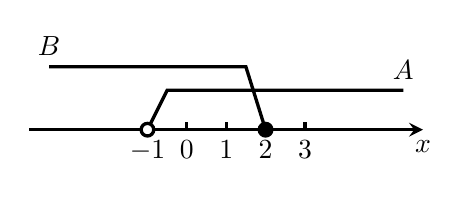
\begin{tikzpicture}[very thick]
\draw[->, >=stealth](-2,0)--(3,0)node[below]{$x$};
\foreach \x/\y in {-.5/-1, 0/0, .5/1, 1/2, 1.5/3}
{
    \draw(\x,0)node[below]{$\y$}--(\x,.1);
}
\draw(-.5,0)--(-.25,.5)--(2.75,.5)node[above]{$A$};
\draw(1,0)--(1-.25,.8)--(-1.75,.8)node[above]{$B$};

\fill[draw] (1,0) circle(.08);
\draw[fill=white] (-.5,0) circle(.08);

    \end{tikzpicture}
    \caption{}
  \end{minipage}
\end{figure}

\begin{example}
设$A=\{x\mid x>-1\}$,$B=\{x\mid x\le 2\}$,求$A\cap B$.
\end{example}

\begin{solution}
    如图1.4所示
    \[A\cap B=\{x\mid x>-1\}\cap\{x\mid x\le 2\}=\{x\mid -1<x\le 2\}\]
\end{solution}


\begin{example}
设$A=\{(x,y)\mid 2x+3y=13\}$,$B=\{(x,y)\mid 3x-y=3\}$,求$A\cap B$.
\end{example}

\begin{solution}
    \[\begin{aligned}
A\cap B&=\{(x,y)\mid 2x+3y=13\}\cap \{(x,y)\mid 3x-y=3\}\\
&=\left\{(x,y)\left|\begin{cases}
    2x+3y=13\\  3x-y=3
\end{cases}\right.\right\}\\
&=\left\{(x,y)\left|\begin{cases}
    x=2\\y=3
\end{cases}\right.\right\}=\{(2,3)\}
    \end{aligned}\]
\end{solution}

\begin{example}
    设$A=\{\text{等腰三角形}\}$,$B=\{\text{直角三角形}\}$,
求$A\cap B$.
\end{example}

\begin{solution}
\[\begin{aligned}
    A\cap B&=\{\text{等腰三角形}\}\cap\{\text{直角三角形}\}\\
    &=\{\text{有两边相等,且有一个角是直角的三角形}\}\\
    &=\{\text{等腰直角三角形}\}
\end{aligned}\]
\end{solution}

\begin{example}
    设$A=\{\text{奇数}\}$,$B=\{\text{正偶数}\}$,$C=\{
\text{小于10的素数}\}$。

求$A\cap C,\; B\cap C,\; A\cap B,\; A\cap \mathbb{N},\; B\cap\mathbb{Q}$
\end{example}

\begin{solution}
\[\begin{aligned}
    A\cap C&=\{\text{奇数}\}\cap\{2,3,5,7\}=\{3,5,7\} \\
     B\cap C&= \{\text{正偶数}\}\cap \{2,3,5,7\}=\{2\}\\
      A\cap B&=\{\text{奇数}\}\cap\{\text{正偶数}\}=\emptyset \\
       A\cap \mathbb{N}&=\{\text{奇数}\}\cap\mathbb{N}=\{\text{正奇数}\} \\
        B\cap\mathbb{Q}&= \{\text{正偶数}\}\cap\mathbb{Q}=\{\text{正偶数}\}=B
\end{aligned}\]
\end{solution}


\subsection{集合的并}
\begin{thm}{实例2}
    高一某班被选拔为校田赛的队员有4名同学:
$a$、$b$
、$c$、$d$, 被选拔为校径赛的队员有3名同学:$a$、$b$、$p$. 
若问这个班被选为校田径队的队员共有哪些同学?这个问题
实质上也是两个集合之间的一种运算问题。
\end{thm}

如果我们用$A$、$B$分别标记这个班被选为田赛和径赛的
队员的同学的集合,就有
\[A=\{a,b,c,d\},\qquad 
B=\{a,b,p\}\]

如果再用$C$标记这个班被选为校田径队的队员的同学的
集合,则
\[C=\{a,b,c,d,p\}\]
很清楚,这里集合$C$的元素是由$A$的元素与$B$的元素“合
并”在一起得到的(注意:合并时相同元素只能看作是一个)。
抽象这种关系就得到:

\begin{thm}{定义5}
    由所有属于集合$A$或属于集合$B$的元素组成的集合,叫做$A$与$B$的\textbf{并集},记作$A\cup B$(读作“$A$并$B$”),即:
    \[A\cup B=\{x\mid x\in A,\; \text{或}x\in B\}\]
“$\cup$”是求两个集合的并集的运算符号。
\end{thm}

这样,被选为校田径队的队员的同学组成的集合可以从
求\{选为田赛队员的同学\}和\{选为径赛队员的同学\}的并集而
得到,即
\[C=A\cup B\]

图1.5中的阴影部分表示集合$A$、$B$的并集$A\cup B$。

由并集的定义容易知道,对于任意两个集合$A$、$B$, 有
\[A\cup A=A,\quad A\cup\emptyset=A,\quad A\cup B\supseteq A, \quad A\cup B\supseteq B\]
\[A\cup B=B\cup A\qquad (\text{交换律})\]

\begin{figure}[htp]
\begin{minipage}{0.45\textwidth}
    \centering
\begin{tikzpicture}[scale=.8]
    \draw[pattern= north east lines](0,0)node[left]{$A$} ellipse(1.5 and 1.5);
    \draw[pattern= north east lines](2,0)node[right]{$B$} ellipse(1.5 and 1.2);
\end{tikzpicture}
    \caption{}
  \end{minipage}
  \hfill 
  \begin{minipage}{0.45\textwidth}
    \centering
    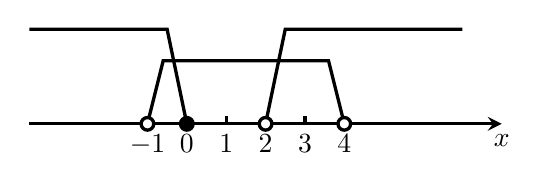
\begin{tikzpicture}[very thick]
\draw[->, >=stealth](-2,0)--(4,0)node[below]{$x$};
\foreach \x/\y in {-.5/-1, 0/0, .5/1, 1/2, 1.5/3, 2/4}
{
    \draw(\x,0)node[below]{$\y$}--(\x,.1);
}

\draw(-2,1.2)--(-.25,1.2)--(0,0);
\draw(1,0)--(1.25,1.2)--(3.5,1.2);
\draw(-.5,0)--(-.3,.8)--(2-.2,.8)--(2,0);

\fill[draw] (0,0) circle(.08);

\foreach \x in {-.5, 2, 1}
{
    \draw[fill=white] (\x,0) circle(.08);
}

    \end{tikzpicture}
    \caption{}
  \end{minipage}
\end{figure}


\begin{example}
    设$A=\{1,2,3,4\}$, $B=\{3,4,5\}$, 求$A\cup B$, 
$A\cap B$.
\end{example}

\begin{solution}
    $A\cup B=\{1,2,3,4,5\},\qquad A\cap B=\{3,4\}$
\end{solution}

\begin{example}
    设$A=\{\text{锐角三角形}\}$,$B=\{\text{钝角三角形}\}$,求$A\cup B$, 
    $A\cap B$.
\end{example}

\begin{solution}
$A\cup B=\{\text{锐角三角形或钝角三角形}\}=\{\text{斜三角形
}\}$

$A\cap B=\emptyset$
\end{solution}

\begin{example}
    设$A=\{x\mid x=2,\;\text{或}x=5\}$,$B=\{
\text{小于5的非负整数}\}$,求$A\cup B$, $A\cap B$.
\end{example}

\begin{solution}
    $\because\quad A=\{2,5\},\quad B=\{0,1,2,3,4\}$

    $\therefore\quad A\cup B=\{0,1,2,3,4,5\},\quad A\cap B=\{2\}$
\end{solution}

\begin{example}
  设$A=\{x\mid -1<x<4\}$,$B=\{x\mid x\le 0,\; \text{或}x>2\}$,  求$A\cup B$, $A\cap B$.
\end{example}

\begin{solution}
    如图1.6,$A\cup B=\mathbb{R}$,$A\cap B=\{x\mid -1<x\le 0,\;\text{或}2<x<4\}$

注意:解这类问题,应画出数轴,直观形象。
\end{solution}


\section*{习题三}
\begin{center}
    \bfseries A
\end{center}

\begin{enumerate}
    \item \begin{enumerate}[(1)]
        \item 设$A=\{1,2,3,4\}$, $B=\{3,4,5,6\}$, 求$A\cap B$, $B\cap A$; 
        \item 设$A=\{1,2,3,4,5,6,7\}$, $B=\{5,6,7\}$, 
   求$A\cap B$, $B\cap A$.
    \end{enumerate}

\item 用适当的符号($\subset,\; \subseteq,\; \supset,\; \supseteq,\; =$)
填空:
\[A\cap B\blank A,\qquad A\cap B\blank B,\qquad A\cap B\blank B\cap A,\qquad \emptyset\blank A\cap B\] 
\item 设$A=\{\text{菱形}\}$,$B=\{\text{矩形}\}$,求$A\cap B$.
\item 设$A=\{\text{锐角三角形}\}$,$B=\{\text{钝角三角形}\}$,求$A\cap B$.
\item \begin{enumerate}[(1)]
    \item 设$A=\{x\mid -2\le x<3\}$, $B=\{x\mid 0\le x<5\}$, 求$A\cap B$
    \item 设$A=\{x\mid x\le -1,\; \text{或}x\ge 3\}$, $B=\{x\mid -4\le x\le 5\}$, 求$A\cap B$
    \item 设$A=\{x\mid 2\le  x<4\}$, $B=\{x\mid x>4\}$,求$A\cap B$
\end{enumerate}
\item 设$A=\{a,b,c,d,d\}$, $B=\{b,c,d,e\}$, $C=\{c,d,e\}$, 求$(A\cap B)\cap C$, $A\cap(B\cap C)$.
\item 求$\{x\mid (x-1)(x+2)=0\}\cap\{x\mid 2x+7=2x-5\}$.


\item 设$A=\{(x,y)\mid 3x+2y=1\}$,$B=\{(x,y)\mid x-y=2\}$,$C=\{(x,y)\mid 2x-2y=3\}$,$D=\{(x,y)\mid 6x+4y=2\}$,$E=\{(x,y)\mid x^2-5xy+6y^2=0\}$

求$A\cap B,\; B\cap C,\; A\cap D,\; C\cap E$.

\item 设$A=\{x\mid x=2k,k\in \mathbb{Z}\}$, $B=\{x\mid x=2k+1,k\in \mathbb{Z}\}$,$C=\{x\mid x=2(k+1), k\in\mathbb{Z}\}$,$D=\{x\mid x=2k-1, k\in\mathbb{Z}\}$

问$A$、$B$、$C$、$D$中哪些集合相等,哪些集合的交集是空
集。
\item 设$A=\{a,b,c\}$, $B=\{b,c,d\}$, 求
$A\cap B$, $A\cup B$, $B\cup A$.

\item 设$A=\{\text{不大于10的非负偶数}\}$, $B=\{\text{6
的正约数}\}$,求$A\cap B$, $A\cup B$.

\item 用适当的符号($\subseteq,\; \subset,\; \supseteq,\; \supset,\; =$)
填空:
\begin{enumerate}[(1)]
    \item $A\blank A\cup B,\quad B\blank A\cup B,\quad A\cup B\blank B\cup A,\quad A\cup B\blank A\cup B$
    \item 若$A\subseteq B$,$A\cup B\blank B,\quad A\cap B\blank A,\quad A\cap B\blank B$
    \item 若把条件$A\subseteq B$加强为
    $A\subset B$, (2)中哪些结论一
    定会改变?
\end{enumerate}

\item 对第5题的条件,分别去求$A\cup B$.
\end{enumerate}

\begin{center}
    \bfseries B
\end{center}

\begin{enumerate}
    \setcounter{enumi}{13}
    \item \begin{enumerate}[(1)]
        \item 已知$A=\{x\mid x=4k-1,\; k\in\mathbb{Z}\}$, $B=\{x\mid x=4k+1,\; k\in\mathbb{Z}\}$, 
        
        求$A\cap B$, $A\cup B$.
        \item 已知$A=\{x\mid x=3k+1,\; k\in\mathbb{Z}\}$, $B=\{x\mid x=3k+2,\; k\in\mathbb{Z}\}$, $C=\{x\mid x=3k-1,\; k\in\mathbb{Z}\}$, 求$A\cup B$, $A\cap B$, $A\cup C$, $A\cap C$, $B\cup C$, $B\cap C$.
    \end{enumerate}

\item 已知$A=\{x\mid x^2-ax+a^2-19=0\}$, $B=\{x\mid x^2-5x+8=2\}$, $C=\{x\mid x^2+2x-8=0\}$,且$A\cap B\supset \emptyset$, $A\cap C=\emptyset$,求$a$的值。
\item 设$A=\{x\mid x^2-2x-8<0\}$,$B=\{x\mid x^2+2x-3>0\}$,$C=\{x\mid x^2-3ax+2a^2<0\}$,求实数$a$的取值范围,使$C\subseteq A\cap B$

\item 设$A=\{x\mid x^2-3x+2<0\}$, $B=\{x\mid x\le a\}$
\begin{enumerate}
    \item 若$A\cap B\ne \emptyset$,求$a$的范围;
    \item 若$A\cap B= \emptyset$,求$a$的范围;
    \item 若$A\subseteq B$,求$a$的范围.
\end{enumerate}
\end{enumerate}

\begin{center}
    \bfseries C
\end{center}

\begin{enumerate}
    \setcounter{enumi}{17}
    \item 对第6题所求得两个结果,你能得出什么结论。对于
    $(A\cup B)\cup C$与$A\cup (B\cup C)$是否也有如上的结果?这说
    明对于交与并两种运算是否存在结合律?并证明你所给
    出的结论。
    \item 利用文氏图解释下列两对集合之间的关系:
    \begin{enumerate}[(1)]
        \item $A\cap (B\cup C)$与$(A\cap B)\cup (A\cap C)$;
    \item $A\cup (B\cap C)$与$(A\cup B)\cap (A\cup C)$.
    \end{enumerate}
    并指出集合中并与交运算是否满足分配律。
    \item 设已知三个有限集合$A,B,C$, 利用文氏图求出$n(A)$, 
    $n(B)$, $n(C)$, $n(A\cap B)$, $n(A\cap C)$, 
    $n(B\cap C)$
    $n(A\cap B\cap C)$和$n(A\cup B\cup C)$之间的关系式。这里$n(A)$
    表示有限集合$A$的元素的个数等。
    \item 向某校高一(1)班学生了解他们对三位歌唱家$A,B,
    C$的演唱艺术是否欣赏。了解的结果是:22人欣赏$A$的
    演唱,25人欣赏$B$的演唱,39人欣赏$C$的演唱,9人对$A,
B$的演唱都欣赏,17人对$A,C$的演唱都欣赏,20人对
$B,C$的演唱都欣赏,6人对三位歌唱家都欣赏,4人对
其中任何人的演唱都不欣赏。全班被问到的共有多少人?
欣赏且只欣赏两位歌唱家演唱的有多少人?
\end{enumerate}


\subsection{集合的补}
在研究集合的问题时,常常把问题中出现的一切集合,
都看作是某个特定集合的子集。如,当我们研究奇数集与偶
数集时,常常把它们看作是\{整数\}这个特定集合的子集。又
如,当我们研究平面$\alpha$上的图形时,又常常把平面$\alpha$上的一切
图形看作是\{平面$\alpha$上的点\}这一特定集合的子集。

\begin{thm}
    {定义6} 在研究集合与集合之间的关系时,如果所给集
合都是某一个特定的集合的子集,这个特定的集合就叫做\textbf{全
集},用符号$I$表示。也就是说,全集含有我们所要研究的各
个集合的全部元素。
\end{thm}

\begin{thm}{定义7}
    已知全集$I$, 集合
    $A\subseteq I$,由$I$中所有不属于$A$的
    元素组成的集合,叫做集合$A$在集合$I$中的\textbf{补集},记作$\overline{A}$(读
    作“$A$补”),即:
\[    \overline{A}=\{x\mid x\in I,\;\text{且}x\notin A\}\]
\end{thm}

图1.7中的长方形内表示
全集$I$, 圆内表示集合$A$, 阴
影部分表示集合$A$在集合$I$中
的补集$\overline{A}$.

\begin{figure}[htp]
    \centering
    \begin{tikzpicture}
\draw[pattern=north east lines](-2,-1) rectangle (1,1);
\draw[fill=white](0,0)node{$A$}circle(.7);        
    \end{tikzpicture}
    \caption{}
\end{figure}

由全集和补集的定义容易知道,对于任意集合$A$, 有
\[A\cup \overline{A}=I,\qquad A\cap \overline{A}=\emptyset,\qquad \overline{\overline{A}}=A\]
其中$\overline{\overline{A}}$表示
$\overline{A}$
在$I$中的补集。

\begin{example}
    设$I=$\{甲班学生\}, $A=$\{甲班男生\}, 那么$\overline{A}=$\{甲班女生\}.
\end{example}

\begin{example}
    设$I=$ \{ 奇数\} , $A=$ \{ 正奇数\}, 那么$\overline{A}=$\{负奇数\}。
\end{example}

\begin{example}
\begin{enumerate}[(1)]
\item 设$I=\mathbb{Q}$, $A=\{x\mid x^2-2=0\}$, 求$\overline{A}$;
\item 设$I=\mathbb{R}$, $A=\{x\mid x^{2}-2=0\}$, 求$\overline{A}$。
\end{enumerate}
\end{example}

\begin{solution}
\begin{enumerate}[(1)]
\item $\because\quad I=\mathbb{Q}$, 方程$x^{2}-2=0$在$\mathbb{Q}$上无解,

$\therefore\quad A= \varnothing$从而$\overline A= \Q$.
\item $\because\quad I=\R$, 方程$x^{2}-2=0$在$\R$ 上有两个根$\pm\sqrt{2}$。

$\therefore\quad \overline{A}=\{x\mid x\in \mathbb{R}, \;\text{且}x\ne\pm\sqrt{2}\}$.
\end{enumerate}
\end{solution}

\begin{example}
    设$I=\{a,b,c,d,e,f\}$, $A=\{a,b\}$, $B=\{b,c,d\}$.
\begin{enumerate}[(1)]
    \item 求$\overline{A}\cap\overline{B}$, $\overline{A\cup B}$, $\overline{A}\cup\overline{B}$, $\overline{A\cap B}$;
    \item 由(1)的计算,你有什么发现?
\end{enumerate}
\end{example}

\begin{solution}
    $\because\quad \overline{A}=\{c,d,e,f\},\quad \overline{B}=\{a,e, f\}$.
\begin{enumerate}[(1)]
    \item $\overline{A}\cap \overline{B}=\{e, f\}$,\quad  $A\cup B=\{a,b,c,d\}$;
    
 $\overline{A\cup B}=\{e,f\}$, \quad $\overline{A}\cup\overline{B}=\{a,c,d,e,f\}$;

$A\cap B=\{b\}$,\quad  $\overline{A\cap B}=\{a,c,b,e,f\}$.

\item 由上述计算结果发现:
\begin{align}
    \overline{A}\cap\overline{B}&=\overline{A\cup B}\tag{*}\\
    \overline{A}\cup\overline{B}&=\overline{A\cap B}\tag{**}
\end{align}
\end{enumerate}

\end{solution}

\begin{note}
\begin{enumerate}
    \item 由上述特定的$A$、$B$计算发现的关于两个集合间的
    交、并、补关系式(*)与(**)具有普遍意义,也就是
    说,对任意的两个集合$A$、$B$, 在确定全集之后它们都是恒等式。这两个公式称为\textbf{摩根定律};
    \item 从左往右使用上述两个公式可把三次运算化为两次
    运算,从而能达到简化计算的目的。
\end{enumerate}
\end{note}

\begin{example}
设$I=\{a,b,c,d,e,f\}$
\begin{enumerate}[(1)]
    \item 若$\overline{A}\cap \overline{B}=\{a,c,e\}$,求$A\cup B$;
    \item 若$\overline{A}\cup \overline{B}=\{a,f\}$,求$A\cap B$;
    \item 若${A}\cup \overline{B}=\{a\}$,求$\overline{A}\cap B$.
\end{enumerate}
\end{example}

\begin{analyze}
    从已知和所求式子的结构特征可以联想到交并补
关系式。
\end{analyze}

\begin{solution}
(1) \textbf{方法1:} 由已知和$\overline{A}\cap\overline{B}=\overline{A\cup B}$,
可得:
\[\overline{A\cup B}=\{a,c,e\}\Longrightarrow A\cup B=\{x\mid x\in I,\; \text{且}x\notin \overline{A\cup B}\}\]
$\therefore\quad A\cup B=\{b,d,f\}$.

\textbf{方法2:} 也可由$\overline{A}\cap \overline{B}=\{a,c,e\}$
两边“取补”得:
\[\overline{\overline{A}\cap \overline{B}} =\overline{\{a,c,e\}}\]
即
\[\overline{\overline{A}}\cup \overline{\overline{B}}=\{b,d,
f\}\Longrightarrow A\cup B=\{b,d,f\}\]

其余两小题由读者完成。    
\end{solution}


\section*{习题四}
\begin{center}
    \bfseries  A
\end{center}

\begin{enumerate}
    \item 已知$\N$为自然数集。
\begin{enumerate}[(1)]
    \item 设$I=\{\text{整数}\}$,求$\overline{\N}$;
\item 设$I=\{\text{非负整数}\}$,求$\overline{\N}$.
\end{enumerate}
  \item 设$I=\R$,$\overline{\Q}=\{\text{无理数}\}$,求$\overline{\Q}$
    的补集$\overline{\overline{\Q}}$

\item 设$I=\{\text{四边形}\}$,$A=\{\text{至少有一组对边平行的四边形}\}$,求$\overline{A}$.

\item 设$A=\{1,3,5\}$,$A=\{2,4,6\}$, $B=\{1,2\}$, 

求$\overline{B}$, $\overline{A\cup B}$, $\overline{A}\cup\overline{B}$.

\item 设$I=\Z$, $A=\{x\mid x=2k,\; k\in\Z\}$, $B=\{x\mid x=2k+1,\; k\in\Z\}$, 

求$\overline{A}$, $\overline{B}$.

\item 设$I=\R$, $A=\{x\mid x\le 6\}$,求
\begin{multicols}{2}
    \begin{enumerate}[(1)]
        \item $A\cap\emptyset$, $A\cup\emptyset$;
        \item $A\cap \R$, $A\cup \R$;
        \item $\overline{A}$;
        \item $A\cap\overline{A}$, $A\cup\overline{A}$.
    \end{enumerate}
\end{multicols}

\item 设$I=\{\text{小于7的非负整数}\}$,$A=\{6的正约数\}$,
$B=\{\text{不大于6的素数}\}$,

求$\overline{A}$, $\overline{A}\cap B$, $A\cup\overline{B}$.

\item 设$I=\{\text{三角形}\}$,$A=\{\text{锐角三角形}\}$,
$B=\{\text{钝角三角形}\}$.

求$\overline{A}\cap\overline{B}$, $\overline{A\cap B}$.
\item 设$I=\{\text{小于20的素数}\}$,$\overline{A}\cap\overline{B}=\{3,7,11,17\}$,求$A\cup B$.
\item 图中的圆形区域分别表示集合$A$、$B$、$C$, 用集合符号写
出下图中的阴影表示的区域:
\begin{figure}[htp]
    \centering
\begin{tikzpicture}
\begin{scope}[xshift=-6cm]
    \draw[fill, pattern=north east lines](-2,-1) rectangle (2,1);
\draw[fill=white](-.6,0)node{$A$} circle(.7);
\draw[fill, pattern=north east lines](0.7,0)node{$B$} circle (.85);
\node at (0,-1.5){(1)};

\end{scope}
\begin{scope}
\node at (0,-1.5){(2)};
\draw(-2,-1) rectangle (2,1);
\draw(0,.3)node[above]{$A$}circle(.5);
\draw(-.4,-.3)node[left]{$B$}circle(.5);
\draw(.4,-.3)node[right]{$C$}circle(.5);

\clip(.4,-.3) circle(.5);
\draw[fill, pattern=north east lines](0,.3)circle(.5);
\end{scope}
\begin{scope}
\clip(-.4,-.3) circle(.5);
\draw[fill, pattern=north east lines](0,.3)circle(.5);
\end{scope}
\end{tikzpicture}
    \caption*{(第10题)}
\end{figure}
\end{enumerate}

\begin{center}
    \bfseries B
\end{center}

\begin{enumerate}\setcounter{enumi}{10}
    \item 已知$I= \{\text{小于20的质数}\}$, $\overline A\cap \overline {B}= \{ 3, 7, 11, 17\}$, 求$A\cup B$.
    \item 已知$I=\{x\mid x=3n,\;  x<30,\; n\in \N\}$,$\overline{A}\cap B=\{6, 15\}$,
    $A\cap\overline{B}=\{3,21\}$,$\overline{A}\cap\overline{B}=\{9,18,24\}$, 利用文氏图求$A,B$.
   
\item    已知$I=\{(x, y)\mid x\in \R,\; y\in \R\}$,$A=\{(x,y)\mid y=
    2x+3\}$,$B=\left\{(x,y)\, \left|\, \frac{y+1}{x+2}=2\right.\right\}$,求:$A\cap\overline{B}$. 
    
\item    利用文氏图验证两个摩根定律。
\end{enumerate}

\section{充要条件}

充要条件\footnote{学习本节前,应适当复习初中学过的有关“命题”的一些内容(可参看
本书附录).}是表述两个命题之间的逻辑关系(谁推出谁)
的概念,在数学中十分重要,有着广泛的应用。

\subsection{充分条件}

若$p\Longrightarrow q$ (这表示由命题$p$成立能推出命题$q$成立),则
称$p$是$q$的充分条件。例如:
\begin{enumerate}[(1)]
    \item 由于两个三角形全等$\Longrightarrow$两个三角形面积相等
    
$\therefore\quad $“两个三角形全等”是“两个三角形面积相等”的充
分条件;
\item 由于$x=y\Longrightarrow x^2=y^2$,

$\therefore\quad $“$x=y$”
是“$x^2=y^2$”
的充分条件;
\item 由于$x\ge y\Longrightarrow \sqrt{(x-y)^2}=x-y$,

$\therefore\quad $“$x\ge y$”
是“$\sqrt{(x-y)^2}=x-y$”的充分条件。
\end{enumerate}

从上述定义可以看出,所谓$p$是$q$的\underline{充分}条件(即
$p\Longrightarrow q$),意指为使$q$成立,具备条件$p$就\underline{足够}了。

\begin{blk}
\begin{enumerate}[(1)]
    \item 你自己举几个充分条件的例子。
    \item 怎样判断$p$是$q$的充分条件?
\end{enumerate}
\end{blk}

\subsection{必要条件}
若$p\Longrightarrow q$,则称$q$
是$p$的必要条件。

\begin{note}
    在初中我们已经学过,命题$p\Longrightarrow q$
与它的逆否命题$\overline{p}\;\Leftarrow \; \overline{q}$
(即$\overline{q}\Longrightarrow\overline{p}$)
是等价的,而$\overline{q}\Longrightarrow\overline{p}$
表明若$q$不成
立,必能推出$p$也不成立。可见,$q$成立是$p$成立所必须的。必
要条件正是由此而得名。
\end{note}

看例子:
\begin{enumerate}[(1)]
    \item 由于
$a=0\Longrightarrow ab=0$,

$\therefore\quad$“$ab=0$”
是“$a=0$”
的必要条件;
\item 由于$a>0$,且$b>0\Longrightarrow a+b>0$,

$\therefore\quad $“$a+b>0$”
是“$a>0$且$b>0$”的必要条件;
\item 由于四边形是正方形$\Longrightarrow$
四边形的四条边相等.

$\therefore\quad $“四条边相等”是“四边形是正方形”的必要条件。
\end{enumerate}

\begin{blk}
\begin{enumerate}[(1)]
    \item 你自己举几个必要条件的例子。
    \item 怎样判断$q$是$p$的必要条件?
\end{enumerate}
\end{blk}


\subsection{充要条件}

若$p$是$q$的充分条件(记作$p\Longrightarrow q$),
且$p$又是$q$的必要条件(记作$q\Longrightarrow p$),
就称\textbf{$p$是$q$的充分必要条件}(简称$p$是$q$的\textbf{充要条件})记作
$p\Longleftrightarrow q$.

例如:
\begin{itemize}
\item “有两个内角相等”是“三角形为等腰三角形”的充要条
件;
\item “对角线互相平分”是“四边形为平行四边形”的充要条件
\item “$x=y$”是“$x-y=0$”的充要条件;
\item “$A\subseteq B$”,且“$B\subseteq A$”是“$A=B$”的充要条件。
\end{itemize}

\begin{blk}
   \begin{enumerate}[(1)]
    \item 你自己举几个充要条件的例子。
    \item 怎样判断$p$是$q$的充要条件?
   \end{enumerate} 
\end{blk}

应该注意,对某个结论来说,条件$p$可能是它的充分条
件,但不是必要条件;或者条件$p$可能是它的必要条件,但
不是充分条件。


例如,“$x>y$”是“$\sqrt{(x-y)^2}=x-y$”的充分条件,但不
是必要条件,因为要使$\sqrt{(x-y)^2}=x-y$
,不一定要有$x>y$,有
$x=y$
也可以。

又如,“$ab=0$”是“$a=0$”
的必要条件,但不是充分条件。
因为由$ab=0$并不一定能推出$a=0$
,还有可能$b=0$.

\begin{blk}
\begin{enumerate}[(1)]
\item 试举是充分条件,但不是必要条件的例子。
\item 试举是必要条件,但不是充分条件的例子。
\item 试举既不是充分条件,又不是必要条件的例子。
\end{enumerate}
\end{blk}

综上所述,充分条件、必要条件和充要条件讲的是两个
命题之间的逻辑关系——\underline{谁推出谁},抓住了这一点就抓住了
这三个概念的本质。

\section*{习题五}
\begin{center}
    \bfseries A
\end{center}

\begin{enumerate}
    \item 将下列各题中的条件先“翻译”成因果关系(用箭头标
    出),再填空:
    \begin{enumerate}[(1)]
    \item 若$p$是$q$的充分条件,则$q$是$p$的\blank 条件;
    \item 若$p$是$q$的必要条件,则$q$是$p$的\blank 条件;
    \item 若$p$是$q$的充要条件,则$q$是$p$的\blank 条件;
    \item 若$A$是$B$的充分条件,$C$是$B$的必要条件,$C$是$D$的
    充分条件,$E$是$D$的必要条件,$F$是$E$的充要条件,
    那么,$A$是$F$的\blank 条件,$E$是$B$的\blank 条件。    
    \end{enumerate}
\item 填空:
\begin{enumerate}[(1)]
    \item $a^{2}=b^{2}$是使$a=b$成立的\blank 条件;
    \item  $a^{3}=b^{3}$是使$a=b$成立的\blank 条件;
    \item 使$ab=0$成立的必要条件是\blank ;
    \item 使$ab=0$成立的充分条件是\blank ;
    \item 使$ab\ne 0$成立的充要条件是\blank ; 
    \item 欲证$A$是$B$的充分条件,由定义,只要证出\blank ;
    \item  欲证$A$是$B$的必要条件,由定义,只要证出\blank ;
    \item 欲证$A$是$B$的充要条件,由定义,只要证出\blank .
\end{enumerate}    
    
\item 若$x\in\R$, 试求使$(1-|x|)(1+x)$
为正数的充要条件。
\item 在下列各题的括号中填写“充分但不必要条件”、“必要但
不充分条件”和“充分必要条件”中的某一种:
\begin{enumerate}[(1)]
    \item “$a^2-1=0$”是“$a-1=0$”的(\qquad\qquad);
    \item “四条边相等”是“四边形是正方形”的(\qquad\qquad);
    \item “$x<5$”是“$x<3$”的(\qquad\qquad);
    \item “$ABCD$是矩形”是“$ABCD$是平行四边形”的(\qquad\qquad);
    \item “同位角相等”是“二直线平行”的(\qquad\qquad);
    \item “$a\ne 0$”是“$ab\ne 0$”的(\qquad\qquad);
    \item “$a^3+b^3$是奇数”是“$a+b$为奇数”($a,b\in \Z$)的(\qquad\qquad);
    \item “$a^{3}-b^{3}$是偶数”是“$a-b$为偶数”($a,b\in \Z)$的(\qquad\qquad).
\end{enumerate}
\end{enumerate}

\begin{center}
    \bfseries B
\end{center}

\begin{enumerate}\setcounter{enumi}{4}
    \item 填空:
\begin{enumerate}[(1)]
    \item “$a>2$”是“$a\ge 2$”的\blank 条件;
    \item “$a,b$不全是0”是“$a,b$全不是0”的\blank 条件;
    \item “到定点距离等于定长的点的集合”是“圆”的\blank 条件;
    \item “$|a-2|\ne 2-a$”是“$a\ge 2$”的\blank 条件.
\end{enumerate}
\end{enumerate}

\section{本章小结}
\subsection{知识结构分析}
见图1.8


\begin{landscape}
\begin{figure}[htp]
    \centering
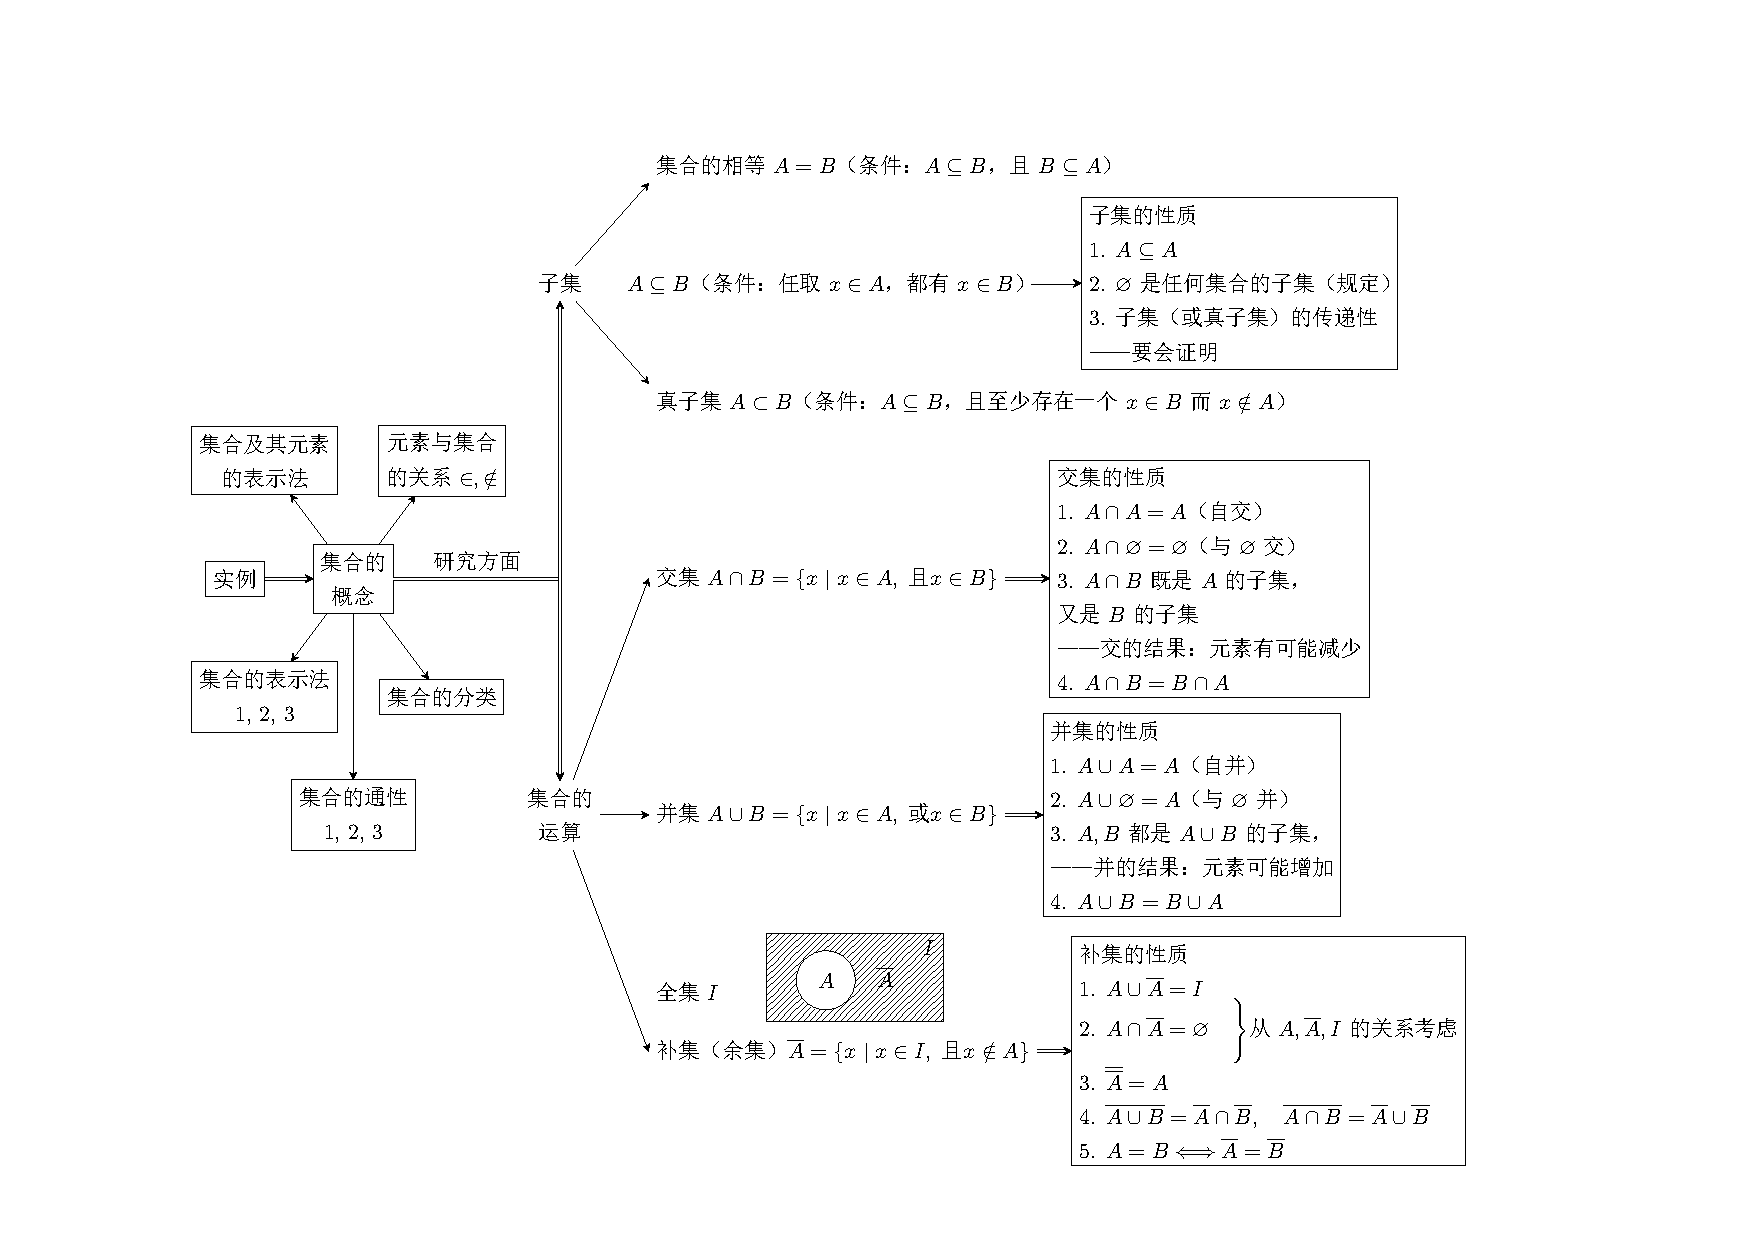
\includegraphics[scale=.7]{fig/fig1-8.pdf}
    \caption{}
\end{figure}
\end{landscape}


\subsection{几点说明}

\begin{enumerate}
    \item 要认真读书。既要对每个概念、符号、结论正确理
    解,正确表达,又要把它们之间逻辑上的联系弄清记牢。这
    就是常言所说的“既看树木,又见森林”。要弄清逻辑上的联
    系,一个有效的办法是根据讲课的顺序画出理论发展的逻辑
    结构图(如图1.8).

    经过这样整理后的知识,由于揭示了知识间的内在联系,理论发展的来龙去脉一目了然,每个知识点在系统中的
地位、作用比较清楚,因而能深化对理论的理解,有利于从
整体上掌握知识。结合这张图:
\begin{enumerate}[(1)]
\item 应能对每个概念正确叙述,并能指出它们在知识
系统中的地位与作用;
\item 应能通过对子、交、并、补集的图示法正确地掌
握它们的性质。
\end{enumerate}

\item 本章中要注意理解、掌握的数学思想有:
\begin{enumerate}[(1)]
 \item 用集合的观点处理问题的思想;
\item 把对象分类讨论的思想;
\item 数与形互相转化的思想。  
\end{enumerate}
\end{enumerate}



\section*{复习题一}
\begin{center}
    \bfseries A
\end{center}

\begin{enumerate}
    \item 已知$A=\{x\mid x\text{是小于6的自然数}\}$, 
    $B=\{x\mid x\text{是小于10的素数(质数)}\}$,  $C=\{x\mid x\text{是24和36的正的公约数}\}$。
    用列举法写出: 
\begin{enumerate}[(1)]
    \item $\{y\mid y\in A,\;\text{且} y\in C\}$;
    \item $\{y\mid y\in A,\;\text{或} y\in B\}$;
    \item $\{y\mid y\in B,\; \text{且}y\notin C\}$.
\end{enumerate}
  \item 已知$A=\{x\mid x=5k+1,\; k\in \Z\}$, $B=\{x\mid x=5k+2,\; k\in \Z\}$, $C=\{x\mid x=5k+3,\; k\in \Z\}$, $D=\{x\mid x=5k-1,\; k\in \Z\}$
  \begin{enumerate}[(1)]
    \item 将集合$A\cup B\cup C\cup D$化简。
    \item 填空:$A\cap B=\blank$, $C\cap D=\blank$。
  \end{enumerate}

\item  用适当的符号($\subset$, $=$, $\supset$)填空:
\begin{enumerate}[(1)]
    \item 已知$A=\{x\mid x=2k+1,\; k\in \Z\}$, $B=\{y\mid y=4k\pm 1,\; k\in \Z\}$, 则$A\blank B$;
    \item 已知$A=\{x\mid x\in\Z,\; x\ne 3n,\; n\in \Z\}$, $B=\{y\mid y=3n\pm 1,\; n\in \Z\}$, 则$A\blank B$;
    \item 已知$A=\{x\mid x=4n,\; n\in \Z\}$, $B=\{x\mid x=6n,\; n\in \Z\}$, 则$A\cap B=\blank $.
\end{enumerate}

\item 已知$A=\{x\mid x=4k,\; k\in \Z\}$, $B=\{x\mid x=4k+2,\; k\in \Z\}$,则$A\cup B=\blank$,$A\cap B=\blank$.

\item 已知$A=\left\{x\left|\; \left|x-\frac{1}{3}\right|>\frac{2}{3}\right.\right\}$, $B=\left\{x\mid |x-2|<3\right\}$,则$A\cap B=\blank$,$\overline{A}\cap \overline{B}=\blank$.

\item 用阴影表示:
\begin{enumerate}[(1)]
    \item $\overline{\overline{A}\cup B}$(其中$A\cap B\ne \emptyset$)
    \item $\overline{C\cap \overline{D}}$(其中$C\cap D\ne \emptyset$)
\end{enumerate}

\item 若$A=\{x\mid 2x^{2}+px+q=0\}$, $B=\{x\mid 6x^{2}+\left(2-p\right)x+5+q=0\}$,且$A \cap B=\left\{\frac{1}{2}\right\}$
,则$A\cup B=\blank$.
\item 设$A=\{-4, 2a-1,a^{2}\}$, $B=\{a-5,1-a,9\}$, 又已知
    $A\cap B=\{9\}$, 求$a$.
\end{enumerate}

\begin{center}
\bfseries B
\end{center}

\begin{enumerate}\setcounter{enumi}{8}
    \item 若$(x-1)^2+\sqrt{y+2}=0$
    的解集为$B$, $A=\{1,-2,3\}$,    则下列关系中正确的是(\qquad )
\begin{multicols}{4}
   \begin{enumerate}[(1)]
    \item $B\subset A$
    \item $B\in A$
    \item $B\cap A=\{1,-2\}$
    \item $B\cap A=\emptyset$
   \end{enumerate} 
\end{multicols}

\item 设$I=\{1,2,5,a^2-3a\}$, $A=\{2,5\}$, $B=\{a,5\}$, $\overline{A\cup B}=\{a-3\}$,$a$有可能取什么值。

\item 已知$I=\R$,$A=\{x\mid |x-a|<4\}$,$B=\{x\mid |x-2|>3\}$,且$A\cup B=\R$,求$a$的范围。
\item 已知$I=\R$,$A=\{x\mid |x-1|\ge a\}$,$B=\left\{x\left|\begin{cases}
    2x-1<3x+5\\ 5x-2<3x+6
\end{cases}\right.\right\}$,且$A\cap B=\emptyset$,求$a$的范围。

\end{enumerate}


\begin{center}
    \bfseries C
\end{center}

\begin{enumerate}\setcounter{enumi}{12}
    \item 设$S$为满足如下条件的自然数构成的集合:
    若$x\in S$, 则$(10-x)\in S$,
\begin{enumerate}[(1)]
\item 试求单元素集$S$;
\item 试求双元素集$S$;
\item 满足条件的集合$S$共有多少个?
\end{enumerate}

\end{enumerate}

